\documentclass[5p]{elsarticle}

\usepackage{amsmath}
\usepackage{commath}
\usepackage{gensymb}
\usepackage[utf8]{inputenc}
\usepackage{listings}
\usepackage[numbered,framed]{mcode}
\usepackage{microtype}
\usepackage[hidelinks]{hyperref}
\usepackage{cleveref}

\DeclareMathOperator{\sech}{sech}

\definecolor{grey}{rgb}{0.9,0.9,0.9}

\lstloadlanguages{Matlab}
\lstset{
  basicstyle=\small,
  breaklines=true,
  frame=single,
  float,
  columns=fullflexible,
  numbers=left,
  stepnumber=2,
  backgroundcolor=\color{grey},
  escapeinside={\%@}{\^^M}
}

% Workaround for bug in elsarticle-num-names.bst
% Reference: http://www.tug.org/pipermail/tex-live/2012-August/032152.html
\makeatletter
\providecommand{\doi}[1]{%
  \begingroup
    \let\bibinfo\@secondoftwo
    \urlstyle{rm}%
    \href{http://dx.doi.org/#1}{%
      doi:\discretionary{}{}{}%
      \nolinkurl{#1}%
    }%
  \endgroup
}
\makeatother

\journal{Journal of Computational Science}

\begin{document}

\begin{frontmatter}

\title{LCS Tool: A Computational Platform for Lagrangian Coherent Structures}

\author{K.~Onu}

\author{F.~Huhn}

\author{G.~Haller\corref{cor}}
\ead{georgehaller@ethz.ch}

\cortext[cor]{Corresponding author}

\address{Institute of Mechanical Systems, ETH Zurich, Switzerland}

\begin{abstract}
% FIXME Reviewer #5, comment #1: Abstract and introduction the objective and contribution of the paper are not clear; several points need to be clarified further.
% FIXME Reviewer #5, comment #2: For readers to quickly catch the contribution in this work, it would be better to highlight major difficulties and challenges, and original achievements to overcome them, in a clearer way in abstract and introduction.
We give an algorithmic introduction to Lagrangian coherent structures (LCSs) using a newly developed computational engine, LCS Tool. LCSs are most repelling, attracting and shearing material lines that form the centrepieces of observed tracer patterns in two-dimensional unsteady dynamical systems. LCS Tool implements the latest geodesic theory of LCSs for two-dimensional flows, uncovering key transport barriers in unsteady flow velocity data as explicit solutions of differential equations. After a review of the underlying theory, we explain the steps and numerical methods used by LCS Tool, and illustrate its capabilities on three unsteady fluid flow examples.
\end{abstract}

\begin{keyword}
Lagrangian coherent structures \sep Mathematical software \sep Non-autonomous dynamical systems \sep Invariant manifolds \sep Mixing \sep Transport barriers \sep Fluid dynamics \sep Ocean surface flows

\PACS 47.10.Fg \sep 47.27.De \sep 47.11.-j \sep 05.45.-a \sep 47.51.+a \sep 47.54.-r \sep 92.10.hf \sep 93.30.Qn \sep 92.10.ab \sep 92.10.Ty \sep 92.10.ak \sep 92.10.A-

\MSC[2010] 37N10 \sep 37B25 \sep 97N80 \sep 37C60 \sep 37B55 \sep 70H33 \sep 76F25
\end{keyword}

\end{frontmatter}

\section{Introduction}

\begin{sloppypar}
% FIXME Reviewer #5, comment #5: Please provide information regarding practical applications of this algorithmic software tool.
Lagrangian Coherent Structures (LCSs) are evolving organizing centres of trajectory patterns in non-autonomous dynamical systems\citep{haller00:_lagran,peacock13:_lagran,haller15:_langr_coher_struc}. Applications of LCSs include oceanic and atmospheric flows\citep{beron-vera13:_objec_agulh,koh02:_hyper}, biological transport problems\citep{wilson09:_lagran_reynol,tallapragada11:_lagran,huhn12:_south_indian_ocean_count_madag}, aeronautics\citep{tang10:_accur_lagran_hong_kong_inter_airpor}, celestial mechanics\citep{gawlik09:_lagran}, crowd dynamics\citep{ali07:_lagran_partic_dynam_approac_crowd}, and aperiodically forced mechanical oscillators\citep{hadjighasem13:_detec_kam}.
\end{sloppypar}

\citet{haller01:_distin} proposed that ridges of the finite-time Lyapunov exponent (FTLE) are heuristic indicators of hyperbolic (i.e., repelling and attracting type) LCSs. A number of examples indeed support this principle\citep{peacock13:_lagran}. Equating FTLE ridges with LCSs, however, would create theoretical inconsistencies, as well as false positives and negatives in hyperbolic LCS detection\citep{haller11:_lagran_coher_struc,norgard12:_secon_lagran_coher_struc}. In addition, the role of the FTLE field in the accurate detection of elliptic (vortex-type) and parabolic (jet-core type) LCSs has remained an open question (but see \citet{beron-vera10:_invar_lagran}).

More recent work has focused on an exact mathematical formulation of the properties defining LCSs\citep{haller11:_lagran_coher_struc,farazmand12:_comput_lagran,haller12:_geodes_theor_trans_barrier_two_dimen_flows,haller13:_coher_lagran,haller14:_adden_coher_lagran,farazmand13:_attrac_lagran,blazevski14:_hyper_ellip_trans_barrier_three}.
In two-dimensional flows, hyperbolic and parabolic LCSs turn out to be stationary curves of the averaged material shear\citep{farazmand14:_shearless}, whereas elliptic LCSs are stationary curves of the averaged strain\citep{haller13:_coher_lagran,haller14:_adden_coher_lagran}.
These variational formulations lead to explicit solutions for LCSs as null geodesics of appropriate Lorentzian metrics.

\begin{sloppypar}
Here we present an algorithmic introduction to geodesic LCS detection.
% FIXME Reviewer #3, comment #4: Add documentation within the github repository to show some reference to the APIs and how users may start to run a his/her own application.
% FIXME Reviewer #4: Please make sure the code is downloadable once the paper is published
We then review the implementation of this approach in a computational engine called LCS Tool\footnote{LCS Tool is available at: \url{http://www.runmycode.org/companion/view/908}}.
This engine is a library of MATLAB functions that extract LCSs from two-dimensional unsteady flows. The examples we present form demonstration scripts distributed with LCS Tool.
\end{sloppypar}

\begin{sloppypar}
Other software for LCS detection exists.
ManGen\citep{lekien03:_time} calculates the FTLE and advects material curves in two-dimensional velocity fields.
It includes a graphical user interface and uses the Message Passing Interface standard for parallel calculations.
Newman\citep{toit10:_trans} calculates the FTLE using dimension independent code.
It assists ridge extraction of FTLE fields and supports analytic and dataset based velocity definitions.
FlowTK\citep{ameli14:_devel_effic_flexib_pipel_lagran} calculates the FTLE in two and three-dimensions on Cartesian and unstructured grids.
The NVIDIA CUDA parallel computing platform is used for fast computations and Kitware's ParaView data analysis and visualization application is used for a user interface.
\end{sloppypar}

\begin{sloppypar}
These packages target the automated generation of FTLE plots to aid the visual assessment of hyperbolic LCSs.
LCS Tool also has functions to generate FTLE plots, but its emphasis is to provide geodesic extraction of LCSs as parametrized material curves, and extend the scope of such extraction to elliptic LCSs.
\end{sloppypar}

\section{Theory}

We consider two-dimensional, finite-time, unsteady velocity fields of the form
\begin{align}
\od{x}{t} = v(x,t), && x \in U \subset \mathbf R^2, && t \in [t_-,t_+].
\label{eq:velocity}
\end{align}
Trajectories of \cref{eq:velocity} are denoted $x(t;t_0,x_0)$, with $x_0 \in U$ denoting their initial position in the open set $U$ at an initial time $t_0 \in [t_-,t_+]$. The flow map is then defined as
\[
F_{t_0}^t(x_0) \equiv x(t;t,x_0),
\]
mapping initial positions to current positions at time $t$. The time interval $[t_-,t_+]$ is part of the definition of the finite-time dynamical system in \cref{eq:velocity}. This interval may be a time scale of interest or the maximum interval over which velocity data is available from simulations or observations.

The right Cauchy-Green strain tensor associated with the flow map is defined as
\begin{equation}
C_{t_0}^t(x_0) = \left[\nabla F_{t_0}^t(x_0)\right]^T \nabla F_{t_0}^t(x_0),
\label{eq:CG}
\end{equation}
measuring Lagrangian strain in the velocity field. This tensor is symmetric and positive definite\citep{truesdell04}. We label the eigenvalues and eigenvectors of $C_{t_0}^t(x_0)$ as follows:
\[
C_{t_0}^t \xi_i = \lambda_i \xi_i, \qquad 0 < \lambda_1 \leq \lambda_2, \quad i = 1,2;
\]
\begin{equation}
\left|\xi_i\right| = 1, \quad \xi_2 = \Omega \xi_1, \quad \Omega = \left(
\begin{array}{rr}
0 & -1\\
1 & 0
\end{array}
\right).
\label{eq:CG_invariants}
\end{equation}

\subsection{Elliptic LCSs}
\label{sec:Elliptic LCSs}

We seek positions of closed material lines at time $t_0$ that prevail as coherent Lagrangian vortex boundaries (or \emph{elliptic LCSs}) over a time interval $[t_0,t]\subset[t_-,t_+]$. \citet{haller13:_coher_lagran,haller14:_adden_coher_lagran} argue that such initial material line positions are closed stationary curves of the averaged strain functional
\[
Q(\gamma) = \frac{1}{\sigma} \int_0^{\sigma} \frac{\sqrt{\langle r'(s),C_{t_0}^t(r(s))r'(s)\rangle}}{\sqrt{\langle r'(s),r'(s)\rangle}} \dif s,
\]
obtained by averaging the tangential strain arising over $[t_0,t]$ along closed material lines parametrized as $r(s)$ with $s \in [0,\sigma].$
Solutions to this variational problem turn out to be closed orbits of one of two parametrized vector-field families
\begin{equation}
\eta_\pm^\lambda = \sqrt{\frac{\lambda_2 - \lambda^2}{\lambda_2 - \lambda_1}} \xi_1 \pm \sqrt{\frac{\lambda^2 - \lambda_1}{\lambda_2 - \lambda_1}}\xi_2,
\label{eq:eta}
\end{equation}
with $\lambda > 0$ playing the role of a parameter. Such closed orbits satisfy the differential equation
\begin{equation}
r' = \eta_\pm^\lambda(r),
\label{eq:etafields}
\end{equation}
which coincide with null geodesics of the Lorentzian metric family 
\[
e_\lambda(u,v) = \left\langle u,\left[D_{t_0}^t(r) - \lambda^2 I\right] v \right\rangle.
\]
For this reason, we refer to the computation of elliptic LCSs as limit cycles of \cref{eq:etafields} as \emph{geodesic detection of elliptic LCSs}.

Any orbit of \cref{eq:etafields} turns out to stretch uniformly under the flow map $F_{t_0}^t$. Specifically, any subset of an orbit of \cref{eq:etafields} increases its arc length precisely by a factor of $\lambda$. For this reason, we refer to trajectories of \cref{eq:etafields} as $\lambda$-lines. Following \citet{haller13:_coher_lagran,haller14:_adden_coher_lagran}, we call the outermost member of a closed family of $\lambda$-lines a coherent Lagrangian vortex boundary.

\subsection{Hyperbolic LCSs}
\label{sec:Hyperbolic LCSs}

Next we consider positions of material lines at time $t_0$ that prevail as most repelling or attracting material lines (or \emph{hyperbolic LCSs}) over a time interval $[t_0,t] \subset [t_-,t_+]$. \citet{farazmand14:_shearless} argue that hyperbolic LCSs are stationary curves of the averaged shear functional
\begin{gather*}
Q(\gamma) = \frac{1}{\sigma} \int_0^\sigma \frac{\langle r'(s),D_{t_0}^t(r(s)) r'(s)\rangle}{\sqrt{\langle r'(s),C_{t_0}^t(r(s)) r'(s)\rangle\langle r'(s),r'(s)\rangle}}\dif s,\\
D_{t_0}^t = \frac12 [C_{t_0}^t \Omega - \Omega C_{t_0}^t],
\end{gather*}
% FIXME Clarify what is meant by _closed_ material lines
obtained by averaging the Lagrangian shear arising over $[t_0,t]$ along closed material lines parametrized as $r(s)$ with $s \in [0,\sigma]$. More precisely, hyperbolic LCSs are stationary curves of $Q(\gamma)$ with respect to fixed-endpoint perturbations. We note that parabolic LCSs (Lagrangian jet cores) are also stationary curves of $Q(\gamma)$, but under variable endpoint perturbations (cf. \citet{farazmand14:_shearless}).

Solutions to this variational problem turn out to be orbits of the $\xi_1$ or $\xi_2$ eigenvector field. Repelling LCSs (\emph{shrink lines}) are obtained as trajectories of the differential equation
\begin{equation}
r' = \xi_1(r),
\label{eq:shrink line}
\end{equation}
and attracting LCSs (\emph{stretch lines}) are obtained as trajectories of the differential equation
\begin{equation}
r' = \xi_2(r).
\label{eq:stretch line}
\end{equation}

Shrink lines and stretch lines coincide with the null geodesics of the Lorentzian metric $h(u,v) = \left\langle u,D_{t_0}^t(r) v \right\rangle$. For this reason, we refer to the computation of hyperbolic LCSs as strongest normally-repelling or normally-attracting orbits of \cref{eq:etafields} as \emph{geodesic detection of hyperbolic LCSs}.

To compute the normal repulsion of shrink lines, we note that an infinitesimal
normal perturbation to a shrink line $\gamma$ at its point $r$ grows under the flow map $F_{t_{0}}^{t}$ by a factor of $\lambda_{2}(r)$ in the direction normal to $F_{t_{0}}^{t}(\gamma).$ Similarly, small normal perturbations to a stretch line decay by a factor $\lambda_{1}(r)$ in the direction normal to the evolving stretch line. 

\section{Numerical methods}

This section describes stepwise the numerical implementation of geodesic detection of elliptic and hyperbolic LCSs based on \cref{eq:etafields,eq:shrink line,eq:stretch line}. \Cref{t:LCS Tool overview} gives an overview of the steps, functions and variable names used in LCS Tool to analyse a flow.

\begin{table}
\begin{enumerate}
\item Define a velocity field, \lstinline!dx = derivative(t,x,p)!
\item Compute Cauchy-Green strain tensor invariants, \lstinline![v,d] = eig_cgStrain(derivative)!
\item Compute $\lambda$-lines, \lstinline![etaPos,etaNeg] = lambda_line(v,d,lambda)!
\item Define Poincare sections, \lstinline!ps!
% FIXME function call below does not reflect LCS Tool usage (e.g. poincare_close_orbit_multi)
\item Detect elliptic LCSs, \lstinline!ellipticLcs = poincare_closed_orbit(etaPos,etaNeg,ps)!
\item Define a local maximization/minimization distance for hyperbolic LCSs \lstinline!lmd!
% FIXME function call below does not reflect LCS Tool usage (e.g. remove_strain_in_shear)
% FIXME seed_curves_from_lambda_max is a poor name for a function that detects hyperbolic LCSs
\item Detect hyperbolic LCSs, \lstinline!hyperbolicLcs = seed_curves_from_lambda_max(v,d,ellipticLcs,lmd)!
\end{enumerate}
\caption{Overview of sequence of computations to detect LCSs with LCS Tool functions.}
\label{t:LCS Tool overview}
\end{table}

\subsection{Computing the invariants of the Cauchy-Green strain tensor}

The first step in calculating elliptic and hyperbolic LCSs is the computation of the Cauchy-Green strain tensor field $C_{t_0}^t(x_0)$, as defined in \cref{eq:CG}. The function performing this calculation in LCS Tool is \lstinline!eig_cgStrain!. The main steps executed by this function are enumerated in \cref{t:Cauchy-Green algorithm}, while \cref{t:eig_cgStrain syntax} summarizes the syntax of \lstinline!eig_cgStrain!.

\begin{table}
\begin{enumerate}
\item Define a Cartesian grid for initial conditions of trajectories. Define an auxiliary grid for differentiating with respect to initial conditions.
\item Solve \cref{eq:velocity} starting from each grid point and auxiliary grid point over the time interval $[t_0,t]$. This gives a discrete approximation to the flow map $F_{t_0}^t(x_0)$.
\item Use finite differencing over the auxiliary grid to compute numerically the derivative of the flow map $DF_{t_0}^t(x_0)$.
\item Compute the Cauchy-Green strain tensor field $C_{t_0}^t(x_0) = \left(DF_{t_0}^t(x_0)\right)^T DF_{t_0}^t(x_0)$, its eigenvalue field $\lambda_{1,2}(x_0)$, and eigenvector fields $\xi_{1,2}(x_0)$ over the initial condition grid.
\end{enumerate}
\caption{Algorithm to calculate the invariants of the Cauchy-Green strain tensor field.}
\label{t:Cauchy-Green algorithm}
\end{table}

\begin{table*}
\begin{center}
\begin{tabular}{|c|p{.7\textwidth}|}
\hline
\multicolumn{2}{|p{.95\textwidth}|}{\lstinline![cgEigenvector,cgEigenvalue] = eig_cgStrain(derivative,domain,timespan,resolution)!}\tabularnewline
\hline
\lstinline!derivative! & function handle for flow velocity equations\tabularnewline
\hline
\lstinline!domain! & $2 \times 2$ array to define flow domain\tabularnewline
\hline
\lstinline!timespan! & $1 \times 2$ array to define flow timespan\tabularnewline
\hline
\lstinline!resolution! & $1 \times 2$ array to define Cauchy-Green strain main grid resolution\tabularnewline
\hline
\lstinline!auxGridRelDelta! & optional scalar between 0 and 0.5 to specify auxiliary grid spacing. Default: $10^{-2}$.\tabularnewline
\hline
\lstinline!eigenvalueFromMainGrid! & optional logical to control whether eigenvalues of Cauchy-Green strain are calculated from main or auxiliary grid. Default: \lstinline!true!.\tabularnewline
\hline
\lstinline!incompressible! & optional logical to specify if incompressibility is imposed. Default: \lstinline!false!.\tabularnewline
\hline
\lstinline!odeSolverOptions! & optional \lstinline!odeset! structure to specify flow map integration parameters\tabularnewline
\hline
\end{tabular}
\caption{Syntax of the function \lstinline!eig_cgStrain!}
\label{t:eig_cgStrain syntax}
\end{center}
\end{table*}

The Cartesian grid of initial conditions mentioned in \cref{t:Cauchy-Green algorithm} is rectangular, with user-defined vertical and horizontal ranges and resolutions. The optimal resolution may be determined by a successive doubling of the initial resolution until convergence of the extracted LCSs is observed visually. If the domain of interest comprises only a few expected LCSs, e.g., one vortex, then a resolution of about 500 grid points along the longest axis usually gives good results. Otherwise, a higher resolution must be chosen.

The auxiliary grid (cf. \cref{t:Cauchy-Green algorithm}) comprises four points placed symmetrically around each point of the Cartesian grid (\cref{f:main and auxiliary grids}). These points are used to achieve increased accuracy in the finite-difference approximation
\begin{gather*}
\nabla F_{t_0}^t(x_0) \approx
\left(\begin{array}{cc}
\alpha_{11} & \alpha_{12}
\\
\alpha_{21} & \alpha_{22}
\end{array}\right)
\\
\alpha_{ij} \equiv \frac{x_i(t;t_0,x_0+\delta x_j) - x_i(t;t_0,x_0-\delta x_j)}{2\vert\delta x_j\vert}
\end{gather*}
of $\nabla F_{t_0}^t$ at a point $x_0$ of the Cartesian grid. Here $\delta x_j$ is a vector of length $\vert\delta x_j\vert > 0$ that points from the Cartesian grid-point $x_0$ in the $j^\text{th}$ coordinate direction (\cref{f:main and auxiliary grids}). Computational improvements arising from the use of the auxiliary grid over simply using the nearest points of the main grid were reported in \citet{farazmand12:_comput_lagran}. Experience suggests setting the auxiliary grid spacing to 1-10\% of the main grid spacing.

\begin{figure}
\begin{center}
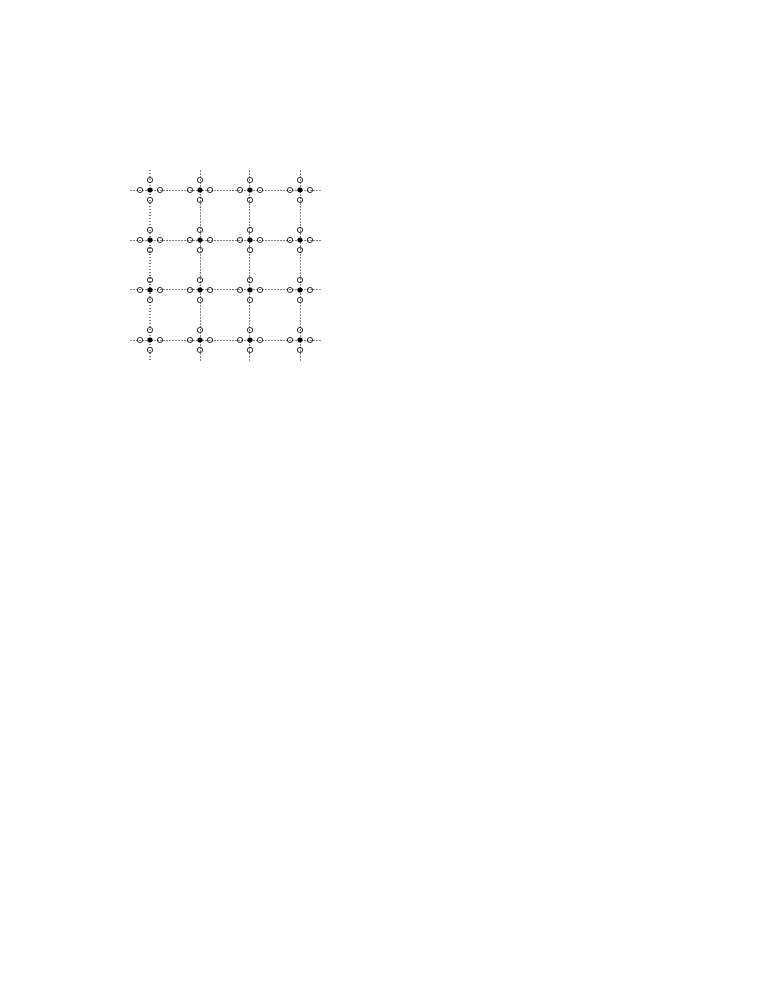
\includegraphics[width=.475\textwidth]{graphics/main_aux_grids}
\end{center}
\caption{Illustration of the main grid (filled circles) and the auxiliary grid (empty circles) used in the computation of the derivative of the flow map in \cref{eq:CG} of the Cauchy-Green strain tensor. The variable \lstinline!auxGridRelDelta! specifies the grid spacing of the auxiliary grid relative to the main grid spacing.}
\label{f:main and auxiliary grids}
\end{figure}

\begin{sloppypar}
The function \lstinline!eig_cgStrain! of LCS Tool provides the option to calculate Cauchy-Green eigenvectors from the auxiliary grid using eigenvalues calculated from the main grid. We have found that for flows defined analytically, the eigenvalues can reliably be calculated from the main grid. For flows defined by datasets, using the auxiliary grid for eigenvalue calculations gives better results.
\end{sloppypar}

\begin{sloppypar}
As mentioned above, a typical main grid for the Cauchy-Green strain tensor comprises $500 \times 500$ points. This means that after the addition of 4 auxiliary grid points around each main grid point, \cref{eq:velocity} must be integrated over 1.25 million initial conditions.
\end{sloppypar}

To avoid excessive computational times in MATLAB, we vectorize \cref{eq:velocity}, i.e., combine its right hand side evaluated over each initial point into a single system of equations. The resulting system is composed of independent blocks of two-dimensional first-order ordinary differential equations. We then use MATLAB's \lstinline!ode45! function to perform trajectory integration from all grid points simultaneously. This calculation typically takes five to ten minutes with default error tolerances.
% FIXME Reviewer #2, comment #3: Add memory use data based on, for example, computations for \cref{f:double gyre lambda LCS convergence}.
A potential drawback of vector form integration is that memory requirements may become excessive at high resolutions. Furthermore, writing the velocity function in vector form is more error-prone than the simpler two-dimensional form.

\begin{sloppypar}
The Cauchy-Green strain tensor generically admits point singularities, i.e., points where $C_{t_0}^t(x_0)$ has repeated eigenvalues. At these points the eigenvectors $\xi_1(x_0)$ and $\xi_2(x_0)$ are no longer well-defined. This generically arises at a finite set of isolated points within the computational domain\citep{delmarcelle94}, and hence lie off the computational grid with probability one.
\end{sloppypar}

\subsubsection{Special case: incompressible velocity fields}

Incompressible flows (i.e. those satisfying $\nabla \cdot v=0$) satisfy the relation $\lambda_1(x_0) \lambda_2(x_0) = 1$ at all points of the computational domain \citep{arnold89:_mathem}. Incompressibility can be computationally imposed by first calculating $\lambda_2(x_0)$, then setting $\lambda_1(x_0) = 1/\lambda_2(x_0)$ and calculating the strain eigenvectors $\xi_2$ from $\lambda_2$, then $\xi_1$ from the relationship in \cref{eq:CG_invariants}. Experience shows that computing $\lambda_i$ in this order gives higher accuracy than in the reverse order \citep{farazmand12:_comput_lagran}.

At some grid points, $\lambda_2 < 1$ may occur due to numerical integration errors. By setting the integration tolerances to smaller values, the number of such grid points is reduced. Enforcing $\lambda_2 \geq 1$ everywhere, however, can incur excessive computational cost. To this end, the function \lstinline!eig_cgStrain! records the number of points with $\lambda_2 < 1$, providing a measure for setting feasible integration tolerances.

\subsubsection{Special case: dataset velocity fields}

Velocity fields defined by datasets require preprocessing before they are used in the numerical integration of \cref{eq:velocity}. This requires spatial and temporal interpolation that enables the evaluation of the velocity function at arbitrary points in $U$ and at arbitrary times between $t_-$ and $t_+$. In \cref{sec:oceandataset}, we present an ocean dataset example with details of possible interpolation functions.

\subsection{Computing elliptic LCSs}

As discussed in \cref{sec:Elliptic LCSs}, positions of elliptic LCSs at time $t_0$ are found as closed orbits of the $\eta_\pm^\lambda$ vector fields defined in \cref{eq:eta}. We find such orbits by integrating \cref{eq:etafields} from points of an appropriately chosen section (Poincare section), and evaluating the first return map (Poincare map) onto this section. A $\lambda$-line returning to its starting point is then an elliptic LCS. The outermost member of a family of closed $\lambda$-lines (obtained by varying $\lambda$) is a coherent Lagrangian vortex boundary\citep{haller13:_coher_lagran,haller14:_adden_coher_lagran}.

The main steps in calculating elliptic LCSs are enumerated in \cref{t:Elliptic LCS algorithm} and described in further detail below. The syntax of elliptic LCS functions in LCS Tool is shown in \cref{t:Elliptic LCS functions}.

\begin{table}
\begin{center}
\begin{enumerate}
\item Position Poincare sections in flow domain to specify initial positions of lambda-lines
\item Integrate $\lambda$-lines tangent to $\eta_\pm^\lambda$ (see \cref{eq:etafields})
\item Calculate Poincare map
\item Find closed orbits for fixed points of the Poincare map
\item Identify outermost closed orbit on each Poincare section
\end{enumerate}
\end{center}
\caption{Algorithm to calculate elliptic LCSs and coherent Lagrangian vortex boundaries.}
\label{t:Elliptic LCS algorithm}
\end{table}

% FIXME Need to update table to account for lambda range
\begin{table*}
\begin{tabular}{|c|p{.7\textwidth}|}
\hline
\multicolumn{2}{|p{.95\textwidth}|}
{\lstinline![shearline.etaPos,shearline.etaNeg] = lambda_line(cgEigenvector,cgEigenvalue,lambda)!}\tabularnewline
\hline
\lstinline!cgEigenvector! & array of Cauchy-Green strain eigenvectors\tabularnewline
\hline
\lstinline!cgEigenvalue! & array of Cauchy-Green strain eigenvalues\tabularnewline
\hline
\lstinline!lambda! & scalar lambda value in \cref{eq:eta}\tabularnewline
\hline \hline
\multicolumn{2}{|p{.95\textwidth}|}{\lstinline![closedOrbits,orbits] = poincare_closed_orbit_multi(domain,resolution,shearline,PSList)!}\tabularnewline
\hline
\lstinline!domain! & array to define flow domain\tabularnewline
\hline
\lstinline!resolution! & $1 \times 2$ array to define main grid resolution for Cauchy-Green strain tensor\tabularnewline
\hline
\lstinline!shearline! & structure of arrays of $\eta_+$ and $\eta_-$ values on main grid\tabularnewline
\hline
\lstinline!PSList! & user-defined structure for Poincare section end-points, number of $\lambda$-lines launched from Poincare section, and maximum closed $\lambda$-line length\tabularnewline
\hline
\lstinline!nBisection! & optional number of bisection steps to refine zero crossings of Poincare map. Default: 5.\tabularnewline
\hline
\lstinline!dThresh! & optional threshold to discard discontinuous zero crossings of Poincare map. Default: $10^{-2}$.\tabularnewline
\hline
\lstinline!odeSolverOptions! & optional \lstinline!odeset! structure to specify $\lambda$-line integration parameters\tabularnewline
\hline
\lstinline!periodicBc! & optional $1 \times 2$ logical array to specify periodic boundary conditions. Default: \lstinline![false,false]!.\tabularnewline
\hline
\end{tabular}
\caption{Syntax for LCS Tool elliptic LCS functions.}
\label{t:Elliptic LCS functions}
\end{table*}

The first step is to define the position of Poincare sections in regions where closed $\lambda$-lines are expected based on a visual analysis of the orbit structure of the $\eta_\pm^\lambda$ vector field. The Poincare section is to be oriented such that the first endpoint is close to the centre of the expected Lagrangian vortex, and the second endpoint is outside this vortex. There is no automated procedure implemented in LCS Tool for the positioning of Poincare sections (see however \citet{karrasch14:_autom_lagran} for a recently developed algorithm). Additionally, the number of lambda-lines launched from the Poincare section, \lstinline!poincareSection.numPoints!, must be defined. A reasonable default value is 100.

The second step is to integrate the $\lambda$-lines  starting from the Poincare section to obtain the corresponding Poincare map. Integration of $\lambda$-lines is performed using the $\eta_\pm^\lambda$ vector fields defined in \cref{eq:eta} over the main grid. The underlying eigenvector fields, $\xi_i(x_0)$, have generic but removable orientation discontinuities, which require monitoring and local reorientation. This process is sketched in \cref{t:variable step integration} and illustrated in \cref{f:variable step integration}. Linear interpolation is used in the interpolation of $\eta_\pm^\lambda$ within a grid element, since using higher-order interpolation would necessitate verifying that there are no orientation discontinuities beyond the four nearest grid points. We identify orientation discontinuities by checking the inner product of the $\eta_\pm^\lambda$ vectors at adjacent grid points. Rotations exceeding 90°, between two such neighbouring vectors are classified as orientation discontinuities and are corrected before linear interpolation. When setting the Cauchy-Green strain tensor main grid resolution, one may find it helpful to calculate a histogram of eigenvector field rotations to ensure that all rotations are well below 90° or almost 180°.

\begin{table}
\begin{enumerate}
\item Linearly interpolate vector field orientation at initial position
\item At next position, check whether vector field has rotated by over 90°, if yes, flip the vector field orientation by 180°.
\item Stop integration when $\lambda$-line returns to Poincare section, $\lambda$-line reaches the domain boundary, or maximum integration length has been reached.
\end{enumerate}
\caption{Algorithm used for variable time step integration of $\lambda$-lines.}
\label{t:variable step integration}
\end{table}

\begin{figure}
\begin{center}
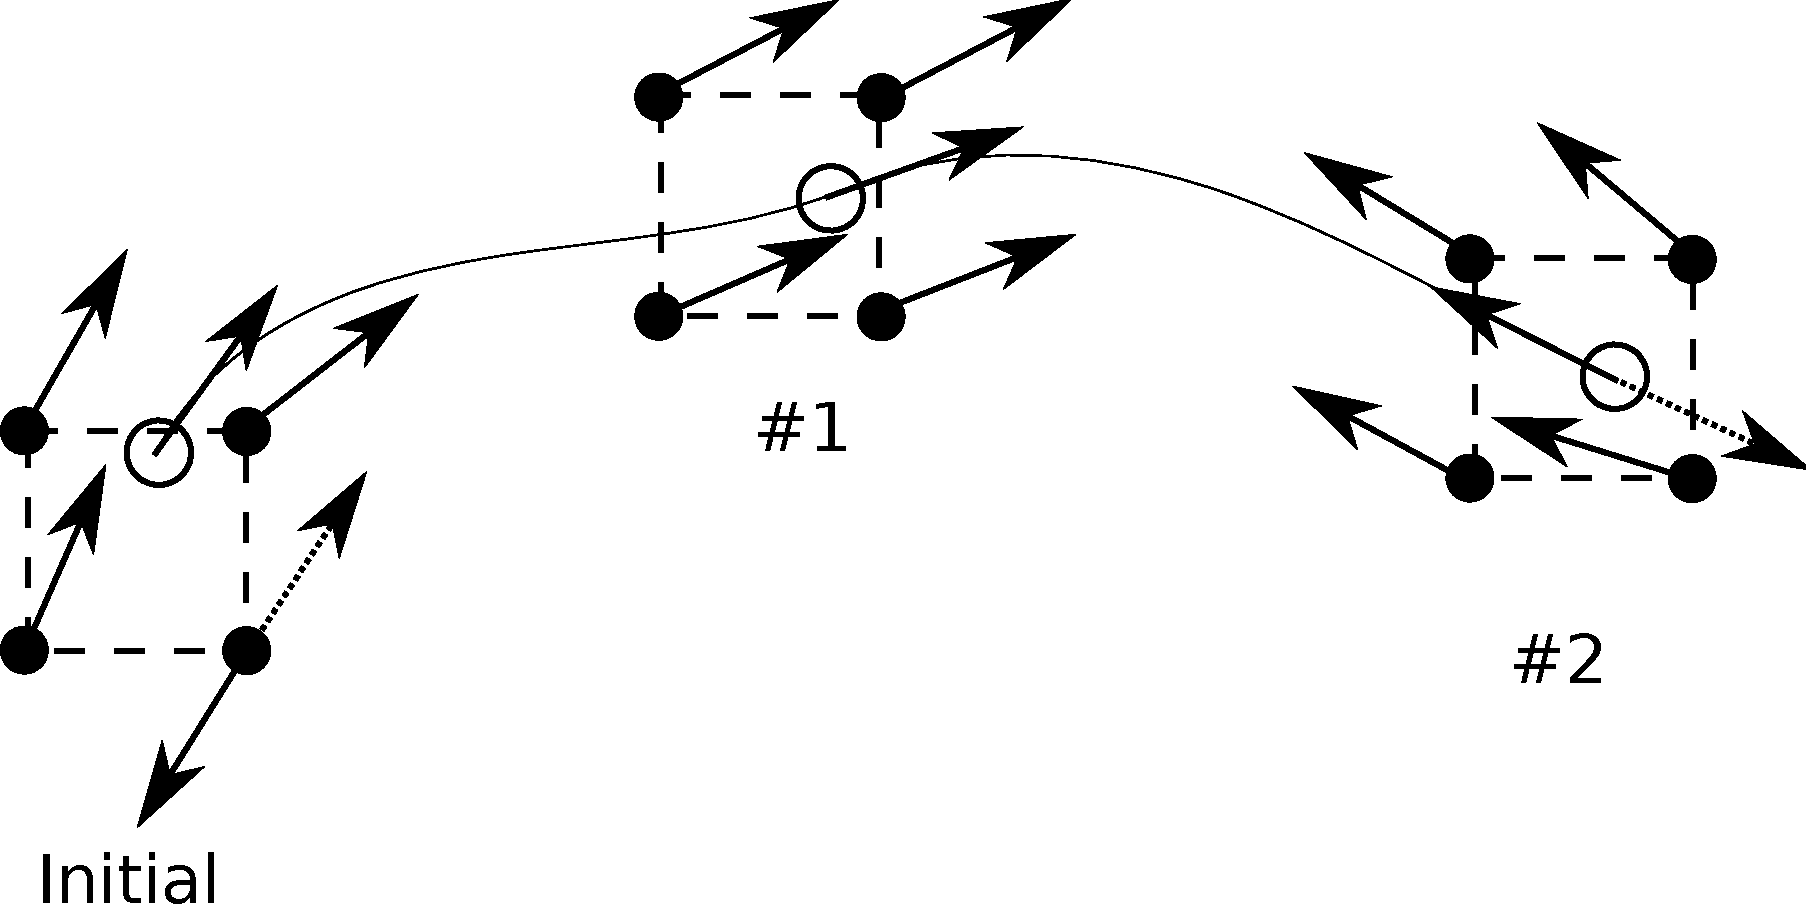
\includegraphics[width=.475\textwidth]{graphics/variable_step_integration}
\end{center}
\caption{Schematic illustration of the variable-time-step $\lambda$-line integration. At the initial point, there is an orientation discontinuity at the lower-right grid point that must be corrected prior to linear interpolation. At point \#1, no orientation discontinuities are present. At point \#2 all interpolated $\eta_\pm^\lambda$ vectors must be rotated by 180° to match the orientation of the trajectory.}
\label{f:variable step integration}
\end{figure}

An example of a Poincare map produced from integration of the $\eta_\pm^\lambda$ field is shown in \cref{f:Poincare return map}. Most orbits will return to the Poincare section and their integration will then be stopped using the ordinary differential equation event detection function of MATLAB. Some orbits may, however, deviate far from the Poincare section and do not return for any reasonable integration time. To control this behaviour, we specify a maximum orbit length, \lstinline!poincareSection.orbitMaxLength!. In practice, viewing the Poincare section as the radius of a circle and setting the maximum $\lambda$-line integration length to twice the circumference gives good results.

In \cref{f:Poincare return map}, circle markers indicate fixed points of the Poincare map, i.e., points where the distance between the final and the initial point of the orbit $P(s) - s$, is zero. The function \lstinline!poincare_closed_orbit_multi! performs the computations. As seen in \cref{f:Poincare return map}, not all zero crossings have circles. This is because LCS Tool uses a filtering parameter, \lstinline!dThresh!, to discard sign changes of $P(s) - s$ that are likely due to numerical sensitivity or a jump discontinuity of the Poincare map. Specifically, the location of each detected zero crossing is first refined by the bisection method. If after a predetermined number of iterations, \lstinline!nBisection!, the two points around the zero crossing still have absolute values above \lstinline!dThresh!, the zero crossing is discarded.  Once all valid closed $\lambda$-lines have been located, the outermost closed $\lambda$-orbit associated with every Poincare section is identified as a coherent Lagrangian vortex boundary.

\begin{figure}
\begin{center}
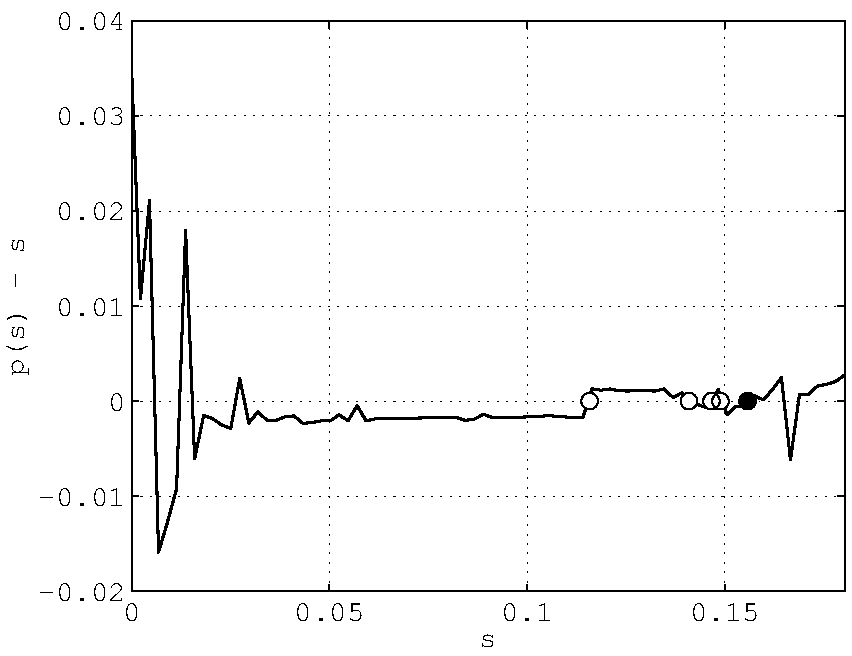
\includegraphics[width=.475\textwidth]{graphics/double_gyre/poincare_return_map}
\end{center}
\caption{Example of a Poincare map obtained for an elliptic LCS. The abscissa, $s$, represents distance along Poincare section. The ordinate, $p(s) - s$, represents distance of Poincare orbit return point from initial position. Circle markers indicate closed orbit positions. The filled circle indicates the outermost fixed point of the Poincare map, marking the intersection of a coherent Lagrangian cortex boundary with the Poincare section.}
\label{f:Poincare return map}
\end{figure}

\subsection{Computing hyperbolic LCSs}

\begin{sloppypar}
As discussed in \cref{sec:Hyperbolic LCSs}, positions of hyperbolic LCSs at time $t_0$ are found as the strongest repelling orbits of the vector field \cref{eq:shrink line} (repelling LCSs), and strongest attracting orbits of the vector field \cref{eq:stretch line} (attracting LCSs). By repulsion and attraction we mean a property of the LCS (as an evolving material line) under the flow map $F_{t_0}^t$. We identify the strongest repelling shrink lines as those crossing a local maximum of the $\lambda_2(x_0)$ field. Similarly, we identify the strongest attracting stretch lines as those crossing a local minimum of the $\lambda_1(x_0)$ field. These local maxima and minima of the appropriate $\lambda_i(x_0)$ eigenvalue field can be thought of as the extensions of the concept of saddle points to the present finite-time, temporally aperiodic flow setting.
\end{sloppypar}

\begin{sloppypar}
The main steps of our hyperbolic LCS detection algorithm are enumerated in \cref{t:Hyperbolic LCS algorithm}. The basic function to compute hyperbolic LCSs in LCS Tool is \lstinline!seed_curves_from_lambda_max! and its syntax is given in \cref{t:seed_curves_from_lambda_max syntax}.
\end{sloppypar}

\begin{table}
\begin{enumerate}
\item Define a local maximization distance.
\item Find all points of the main grid that are local maxima of $\lambda_2$ within a circle whose radius is the local  maximization distance.
\item Define a maximum shrink line length
\item Integrate a shrink line forward and backward according to \cref{eq:shrink line} and using the largest $\lambda_2$ local maximum as the initial position. Integrate until the shrink line has attained the maximum shrink line length, or until it has reached the domain boundary.
\item Flag any remaining local maxima of $\lambda_2$ within the maximization distance of the shrink line as ineligible initial positions for subsequent shrink lines
\label{i:flag maxima}
\item Continue integrating shrink lines using local maxima of $\lambda_2$ as initial positions until no eligible local maxima of $\lambda_2$ remain.
\item Remove all shrink line segments within elliptic LCSs.
\end{enumerate}
\caption{Algorithm to calculate initial positions of repelling LCSs at time $t_0$. The algorithm for attracting LCSs is similar.}
\label{t:Hyperbolic LCS algorithm}
\end{table}

\begin{table*}
\begin{center}
\begin{tabular}{|c|p{.7\textwidth}|}
\hline
\multicolumn{2}{|p{.95\textwidth}|}
{\lstinline![curvePosition,curveInitialPosition] = seed_curves_from_lambda_max(distance,cgEigenvalue,cgEigenvector,flowDomain,flowResolution)!}\tabularnewline
\hline
\lstinline!distance! & threshold distance for placement of $\lambda_2(x_0)$ maxima\tabularnewline
\hline
\lstinline!cgEigenvalue! & array of Cauchy-Green strain eigenvalues\tabularnewline
\hline
\lstinline!cgEigenvector! & array of Cauchy-Green strain eigenvectors\tabularnewline
\hline
\lstinline!flowDomain! & $2 \times 2$ array to define flow domain\tabularnewline
\hline
\lstinline!flowResolution! & $1 \times 2$ array to define Cauchy-Green strain main grid resolution\tabularnewline
\hline
\lstinline!periodicBc! & optional $1 \times 2$ logical array to specify periodic boundary conditions. Default: \lstinline![false,false]!.\tabularnewline
\hline
\lstinline!nMaxCurves! & optional maximum number of curves (i.e. shrink lines or stretch lines) to generate. Default: \lstinline!numel(cgEigenvalue)!.\tabularnewline
\hline
\lstinline!odeSolverOptions! & optional \lstinline!odeset! structure to specify flow map integration parameters\tabularnewline
\hline
\end{tabular}
\end{center}
\caption{Syntax of the function \lstinline!seed_curves_from_lambda_max!}
\label{t:seed_curves_from_lambda_max syntax}
\end{table*}

In classical, infinite-time dynamical systems, elliptic and hyperbolic invariant manifolds cannot intersect, as the trajectories in their intersection would then have to follow two different asymptotic behaviours simultaneously. In finite-time dynamical systems, hyperbolic LCSs may well intersect elliptic LCSs, with hyperbolic LCSs continuing to act as cores of mixing patterns observed in the interior of elliptic LCSs. Motivated by convention and for clarity in visualization, however, the default setting of LCS Tool removes hyperbolic LCS segments from the interior of elliptic LCSs. These removed segments can be turned back on demand, as shown in \cref{f:ocean_dataset_colortracer}.

\begin{figure}
\centering
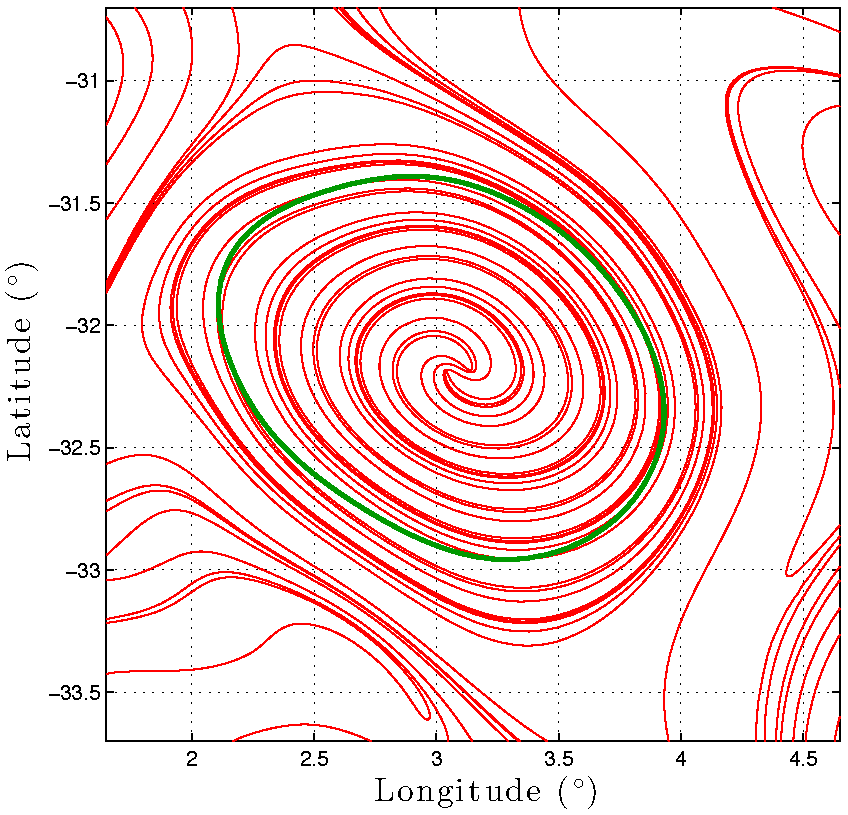
\includegraphics[width=.475\textwidth]{graphics/ocean_dataset/LCS_fwd_coherent_eddy}
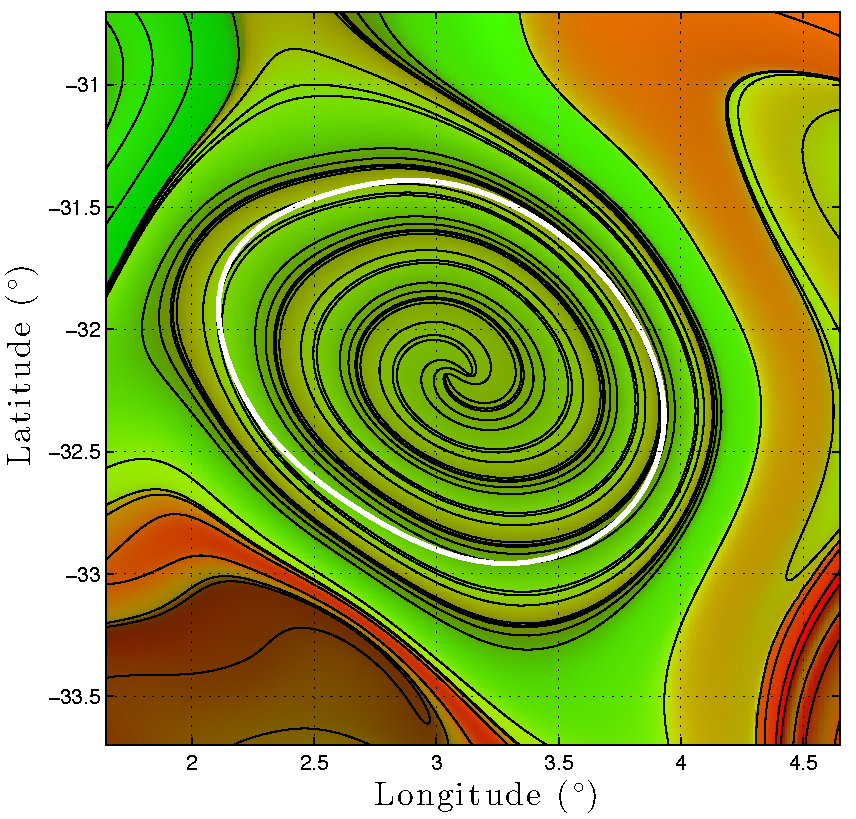
\includegraphics[width=.475\textwidth]{graphics/ocean_dataset/LCS_fwd_colortracer}
\caption{(Top) Elliptic LCS (green) with repelling LCSs (red) continuing into its interior. (Bottom) Final positions $x(t) = (x_1(t),x_2(t)) = F_{t_0}^t(x_0)$ of tracer particles. $x_1(t)$ position encoded in red and $x_2(t)$ position encoded in green. Note the continued impact of the repelling hyperbolic LCSs (black) on tracer patterns inside the elliptic LCS (white).}
\label{f:ocean_dataset_colortracer}
\end{figure}

\section{Examples}

This section presents the use of LCS Tool in three examples: a double gyre, a jet, and an oceanic geostrophic flow. The examples are available as scripts in the demo folder of LCS Tool. Executing these scripts can help readers follow LCS Tool computations.

% FIXME Performance also described in Conclusions section
The scripts call LCS Tool functions.
These functions are written to achieve balance between ease of use and performance.
% FIXME List demo script run-times in minutes in a table
Running the demo scripts takes on the order of minutes.

\subsection{Double gyre}
The double gyre is a model for a time-dependent two gyre system observed in geophysical flows \citep{shadden05:_defin_lagran_lyapun}. The model consists of two counter rotating sinusoidal vortices with a harmonically oscillating line in-between. Lagrangian particle motions satisfy the non-autonomous dynamical system
\begin{equation}
\begin{split}
\od{x}{t} = -\pi A \sin[\pi f(x,t)] \cos(\pi y),\\
\od{y}{t} = \pi A \cos[\pi f(x,t)] \sin(\pi y) \pd{f(x,t)}{x},\\
f(x,t) = \epsilon \sin(\omega t) x^2 + [1 - 2 \epsilon \sin(\omega t)] x.
\end{split}
\label{eq:double gyre derivative equations}
\end{equation}
The MATLAB function describing this velocity field is given in \cref{l:double gyre derivative}, specifying the right hand side of the particle ordinary differential equation in a way that supports vectorized integration.

% FIXME Reviewer #2, comment #8: Check all code listings for awkward splits across pages and line-splits (e.g. semicolon on own line and array indices)
% FIXME Reviewer #5, comment #3: Format manuscript carefully with regards to code listings
\begin{lstlisting}[caption={Double gyre derivative function corresponding to \cref{eq:double gyre derivative equations}.},label=l:double gyre derivative]
function derivative_ = derivative(t,x,epsilon,amplitude,omega)

idx1 = 1:2:numel(x)-1;
idx2 = 2:2:numel(x);

a = epsilon*sin(omega*t);
b = 1 - 2*epsilon*sin(omega*t);
forcing = a*x(idx1).^2 + b*x(idx1);

derivative_ = nan(size(x));

derivative_(idx1) = -pi*amplitude*sin(pi*forcing).*cos(pi*x(idx2));
derivative_(idx2) = pi*amplitude*cos(pi*forcing).*sin(pi*x(idx2)).*(2*a*x(idx1) + b);
\end{lstlisting}

In what follows, the parameter values are: $A = 0.1$, $\epsilon = 0.1$, $\omega = \pi/5$. The flow timespan is $t \in [0,10]$ and the domain is $x \in [0,2]$, $y \in [0,1]$. By examining the FTLE field (which LCS Tool can provide), we position Poincare sections to capture elliptic LCSs. An LCS Tool demo script to perform this operation is given in \cref{l:double gyre elliptic LCS} where two Poincare sections are defined (\cref{ll:double gyre poincareSection(1),ll:double gyre poincareSection(2)}). The free stretching parameter $\lambda$ (\cref{eq:etafields}) is varied over the range $[0.93,1.07]$ with increments of $0.01$ (\cref{ll:double gyre lambdaRange}).
% FIXME The cited loop contains ellipses (...), that hide important code and should become an LCS Tool function
In a loop (\crefrange{ll:double gyre lambda loop start}{ll:double gyre lambda loop end}), closed orbits for all predefined $\lambda$ values are computed and the outermost closed orbit is kept as the Lagrangian vortex boundary.
% FIXME Small tolerances (i.e. strict tolerances) should make convergence difficult not easy, so the word "facilitate" in the sentence below seems illogical.
In this script, we have chosen small values for the error tolerances of the integration of the Cauchy-Green strain tensor (\cref{ll:double gyre cgStrainOdeSolverOptions}) and $\lambda$-lines (\cref{ll:double gyre lambdaLineOdeSolverOptions}) to facilitate convergence.

\lstinputlisting[caption={LCS Tool commands for double gyre elliptic LCSs. Subset of the LCS Tool script \lstinline!demo/double_gyre/hyperbolic_shear_lcs.m!},
                 label=l:double gyre elliptic LCS]{listings/double_gyre/elliptic_lcs_subset.m}

In \cref{f:double gyre lambda LCS convergence}, the resolution of the  Cauchy-Green strain tensor is varied from $500 \times 250$ to $1000 \times 500$. The location of the outermost closed $\lambda$-line changes insignificantly, demonstrating convergence. For all tested resolutions, the $\lambda$ values of the outermost closed orbits match.
% FIXME Should reduce lowest resolution used to demonstrate problems if selected resolution is too low
This also suggests that the lowest tested resolution, $500 \times 250$, is sufficient to identify elliptic LCSs.

\begin{figure}
\centering
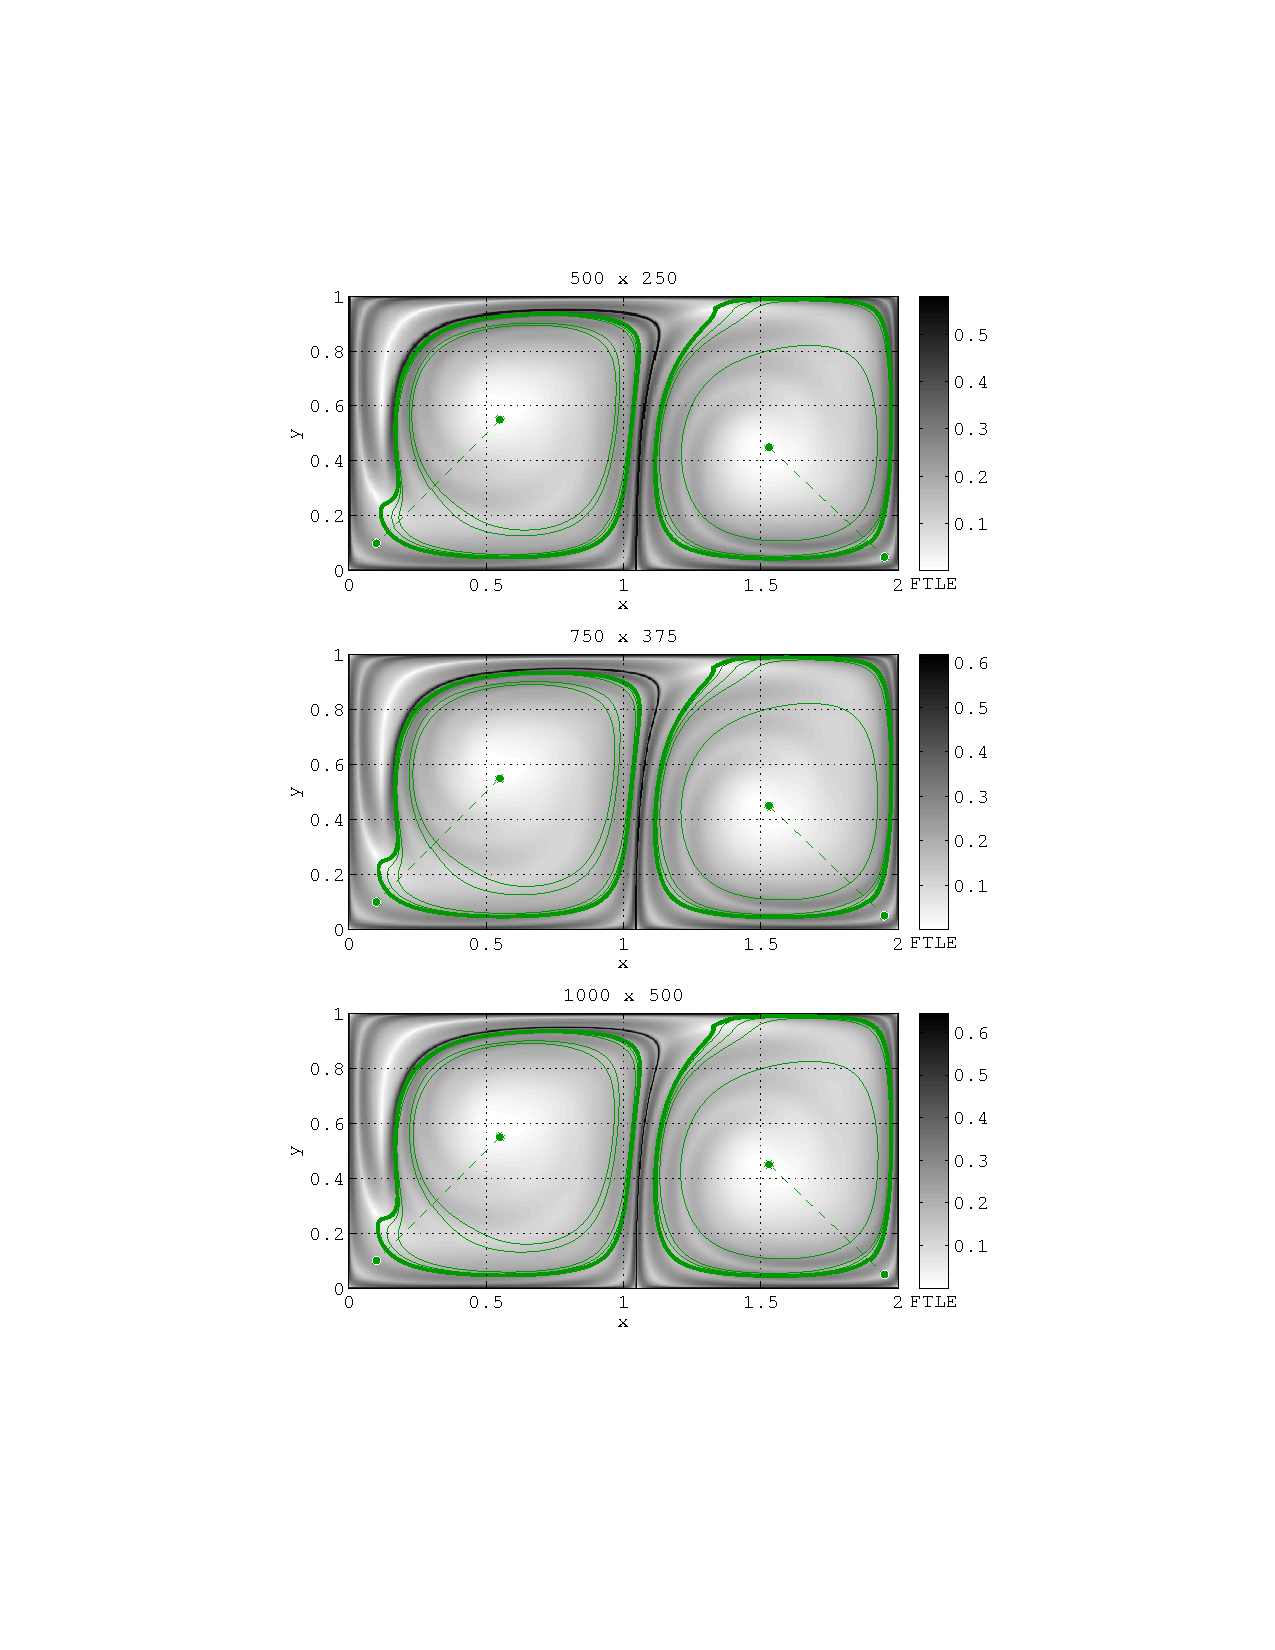
\includegraphics[width=.475\textwidth]{graphics/double_gyre/lambda_lcs_convergence}\caption{Convergence of closed $\lambda$-lines for increasing main-grid resolution in the double-gyre model. The outermost closed $\lambda$-line (bold green line) is the vortex boundary. (Top) {[}500x250{]}, $\lambda$-values
of closed orbits from interior to exterior, left gyre: $\lambda=(0.97, 0.98, 0.99, 1.00, 1.01)$, right gyre: $\lambda=(1.00, 1.01, 1.02, 1.03, 1.04)$; (Middle) {[}750x375{]}, left: $\lambda=(0.97, 0.98, 0.99, 1.00, 1.01)$, right: $\lambda=(1.00, 1.01, 1.02, 1.03, 1.04, 1.05)$; (Bottom) {[}1000x500{]}, left: $\lambda=(0.97, 0.98, 0.99, 1.00, 1.01)$, right: $\lambda=(1.00, 1.01, 1.02, 1.03, 1.04, 1.05)$.}
\label{f:double gyre lambda LCS convergence}
\end{figure}

\begin{sloppypar}
\Cref{f:double gyre lambda hyperbolic LCS} shows the complete picture of elliptic and hyperbolic LCSs of the double gyre at this resolution. \Cref{l:double gyre lambda strain stretch LCS} lists the corresponding LCS Tool commands. The maximal length of shrink lines and stretch lines, \lstinline!shrinkLineMaxLength! and \lstinline!stretchLineMaxLength!, is set to $20$, a multiple of the domain size, since the hyperbolic LCSs may wind around vortices several times. 
\end{sloppypar}

As usual, the local maximization distance is set larger for stretch lines than for shrink lines (cf. \cref{ll:shrinkLineLocalMaxDistance} and \cref{ll:stretchLineLocalMaxDistance}). The purpose of the maximization distance is to obtain spatially separated LCSs and to avoid a dense tangle of lines that basically indicates the same hyperbolic LCS (cf. \cref{t:Hyperbolic LCS algorithm}, \cref{i:flag maxima}). Setting the local maximization distance for stretch lines larger than for shrink lines allows obtaining a comparable number of stretch lines and shrink lines overall in the flow domain (recall that hyperbolic LCS seed points are discarded if they are within the local maximization distance of an existing hyperbolic LCS). Shrink lines are locally tangent to ridges of $\lambda_2$ maxima, whereas stretch lines are locally normal to these ridges. Setting the local maximization distance of stretch lines and shrink lines equal would therefore produce a greater number of stretch lines than shrink lines overall.

% FIXME Reviewer #5, comment #4: There is too much source code in the main content such as cref{l:double gyre lambda strain stretch LCS,l:Bickley jet elliptic hyperbolic LCS subset,l:ocean data elliptic hyperbolic lcs}. They could be arranged as an appendix at the end.
\lstinputlisting[
        caption={LCS Tool commands for double gyre hyperbolic LCSs. Subset of the LCS Tool script \lstinline!demo/double_gyre/hyperbolic_shear_lcs.m!},
        label=l:double gyre lambda strain stretch LCS]
        {listings/double_gyre/hyperbolic_lcs_subset.m}

\begin{figure}
\centering
% FIXME Reviewer #2, comment #6: Improve appearance of $lambda$ extrema (white dots)
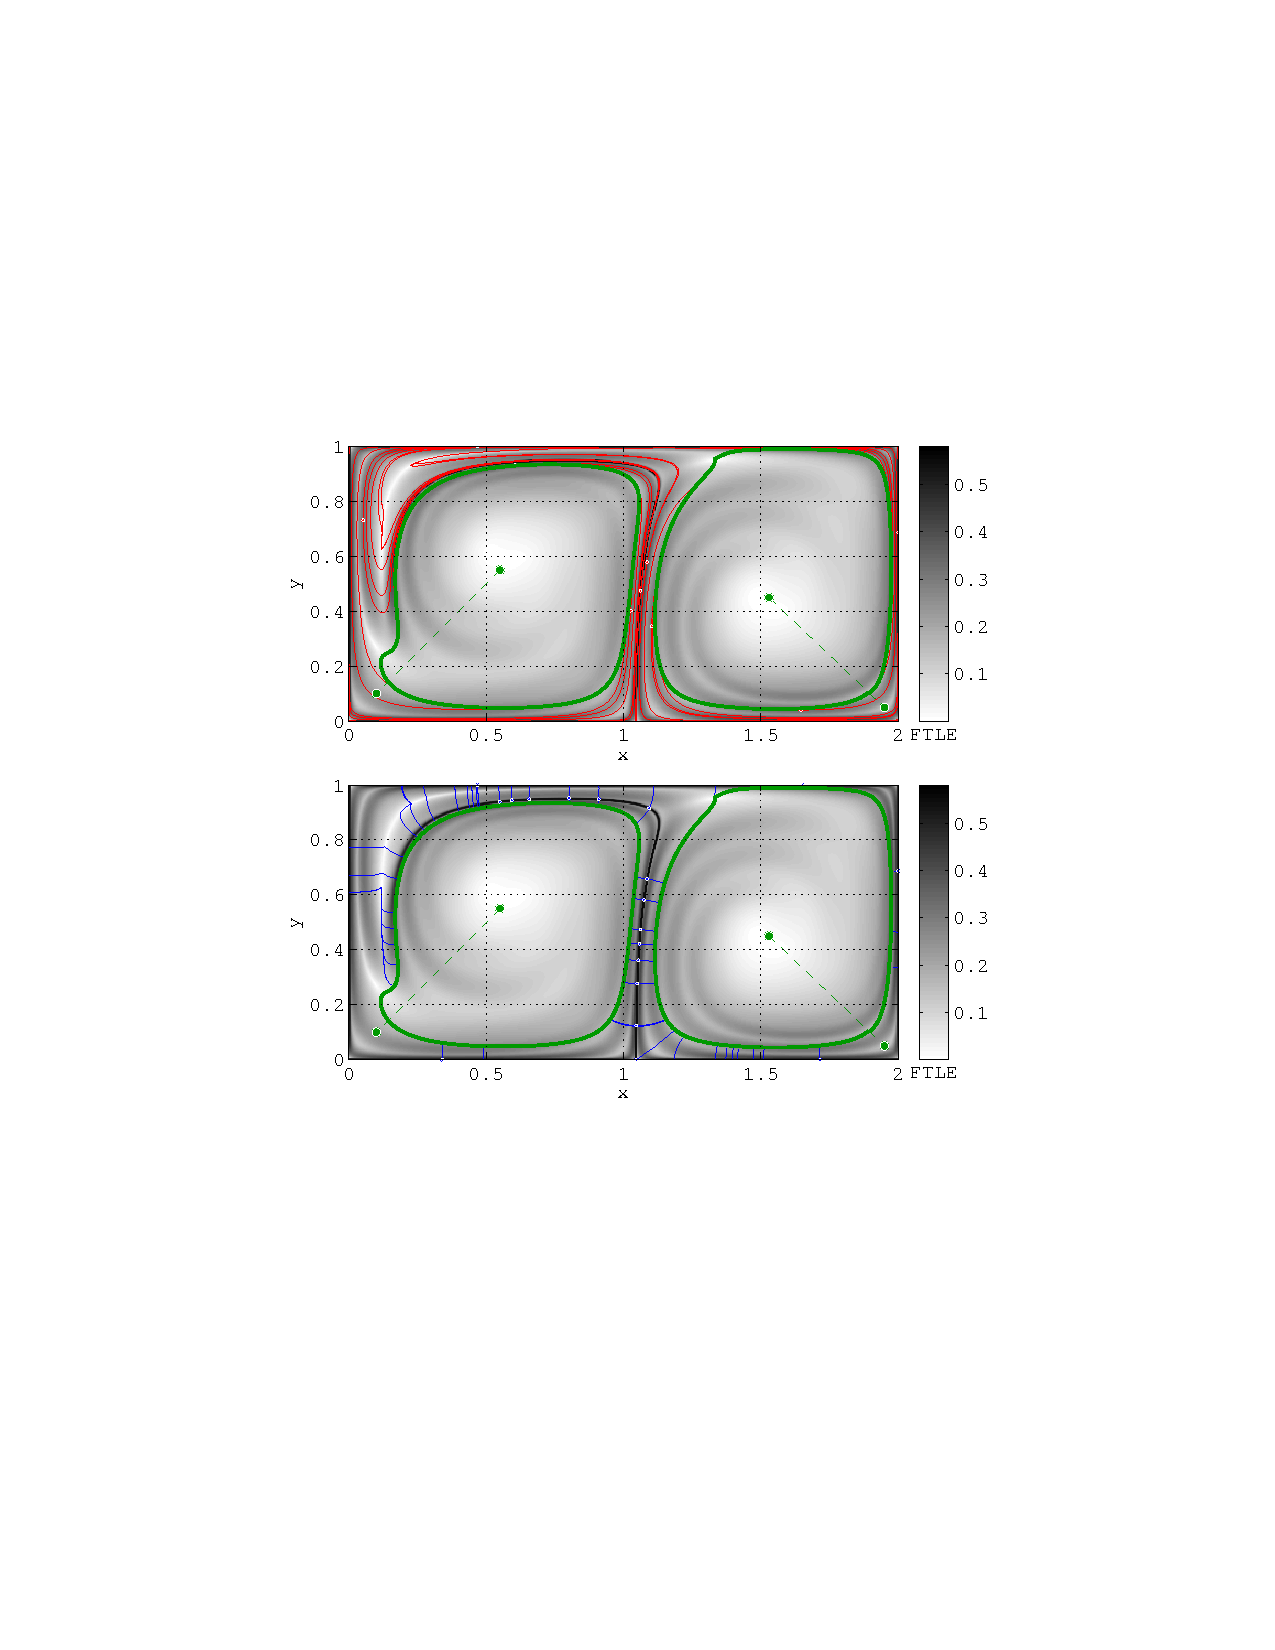
\includegraphics[width=.475\textwidth]{graphics/double_gyre/lambda_hyperbolic_lcs}
\caption{
LCSs in the double gyre.
Resolution is $[500\times250]$.
Elliptic LCSs are green, shrink line LCSs are red and stretch line LCSs are blue.
White dots indicate $\lambda_2$ maxima for shrink lines and $\lambda_1$ minima stretch lines.
FTLE shown in the background.
$\lambda = 1.00$ and $1.04$ for the left and the right gyre.
$\lambda \in [0.93,1.07]$, $\Delta\lambda = 0.01$.
}
\label{f:double gyre lambda hyperbolic LCS}
\end{figure}

\subsection{Bickley jet}

The Bickley jet models a meandering zonal jet flanked above and below by
counter rotating vortices. This is an idealized model of geophysical flows such as the Gulf Stream and the polar night jet perturbed by a Rossby wave\citep{castilloNegrete93:_chaot_rossb,beron-vera10:_invar_lagran}.

The velocity is given by $v(x,y,t) = (-\partial_y \psi, \partial_x \psi)$ where
\begin{gather*}
\psi(x,y,t) = \psi_0(x,y) + \psi_1(x,y,t),\\
\psi_0(x,y) = c_3 y - U L_y \tanh\frac{y}{L_y} + \epsilon_3 U L_y \sech^2\frac{y}{L_y} \cos k_3 x,\\
\psi_1(x,y,t) = U L_y \sech^2\frac{y}{L_y} \Re\left[\sum_{n=1}^2 \epsilon_n f_n(t) e^{i k_n x}\right].
\end{gather*}
As a forcing function, we choose a solution running on the chaotic attractor of the damped and forced Duffing oscillator, specifically
\begin{gather*}
\od{\phi_1}{t} = \phi_2,\\
\od{\phi_1}{t} = -0.1 \phi_2 - \phi_1^3 + 11 \cos(t),\\
f_{1,2}(t) = 2.625 \times 10^{-2} \phi_1(t/6.238 \times 10^5)
\end{gather*}
The parameter values we use are: $U = 62.66$, $c_2 = 0.205 U$, $c_3 = 0.461 U$, $L_y = 1.77 \times 10^6$, $\epsilon_1 = 0.0075$, $\epsilon_2 = 0.04$, $\epsilon_3 = 0.3$, $L_x = 6.371 \times 10^6 \pi$, $k_n = 2 n \pi/L_x$, $\sigma_1 = 0.5 k_2 (c_2 - c_3)$, $\sigma_2 = 2 \sigma_1$.

% FIXME Reviewer #2, comment #7: sentence reads awkwardly
The integration time is $T = 4L_x/U$, a multiple of the eddy turnover time. \Cref{l:Bickley jet elliptic hyperbolic LCS subset} shows the LCS Tool commands in which the chaotically perturbed velocity is defined (\crefrange{ll:Bickley jet velocity definition start}{ll:Bickley jet velocity definition end}), periodic boundary conditions are imposed in the x-direction (\cref{ll:Bickley jet periodicBc}), and five Poincare sections are defined where we expect coherent vortices (\crefrange{ll:Bickley jet Poincare start}{ll:Bickley jet Poincare end}).
$\lambda$-values for closed orbit detection are varied over the range $[0.80,1.20]$ with a step of $0.01$.

\Cref{f:Bickley jet LCS} shows elliptic and hyperbolic LCSs of the Bickley jet with the FTLE in the background.

\lstinputlisting[
        caption={LCS Tool commands for Bickley jet elliptic and hyperbolic LCSs. Subset of the LCS Tool script \lstinline!demo/bickley_jet/hyperbolic_shear_lcs.m!},
        label=l:Bickley jet elliptic hyperbolic LCS subset]
        {listings/bickley_jet/elliptic_hyperbolic_lcs_subset.m}

\begin{figure}
\centering
% FIXME Shrink line LCS figure does not treat periodic boundary condition correctly
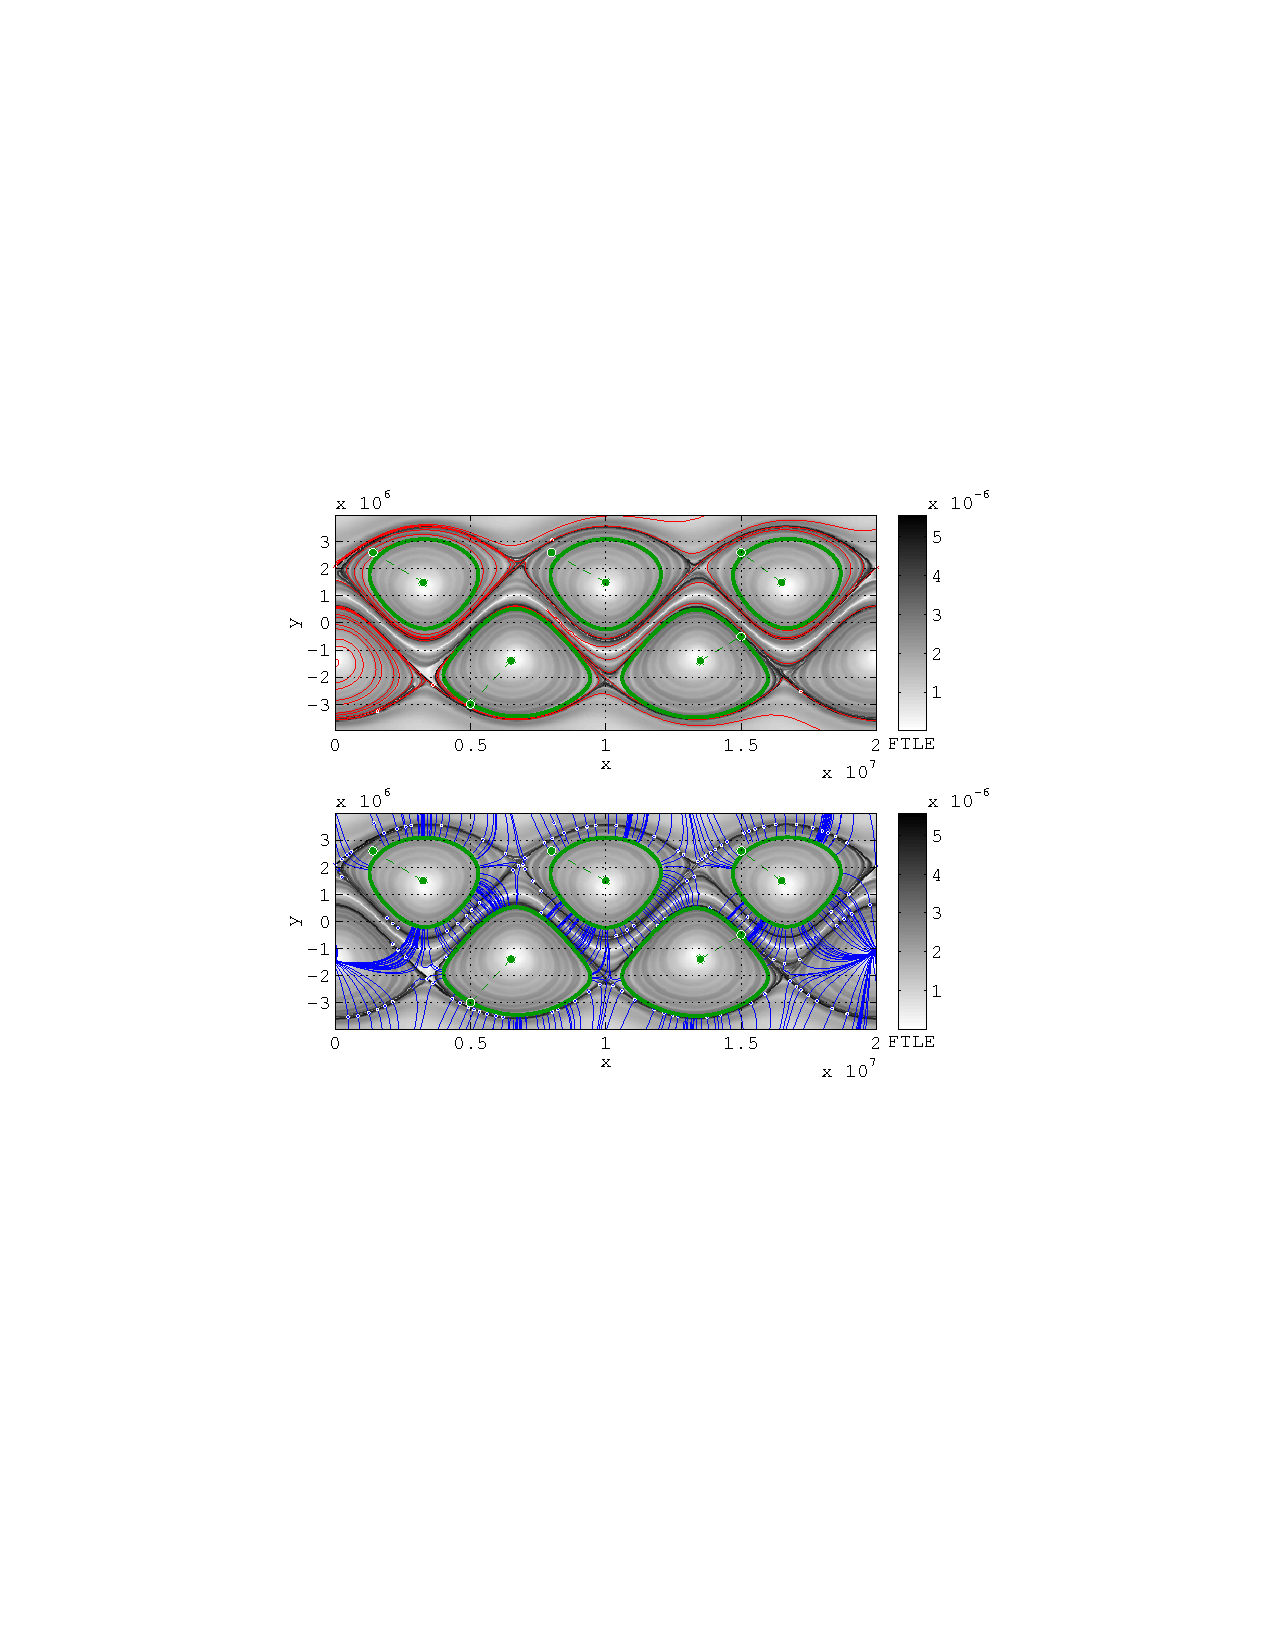
\includegraphics[width=.475\textwidth]{graphics/bickley_jet/lambda_hyperbolic_lcs}
\caption{
LCSs in the Bickley jet.
Resolution is $[500 \times 276]$.
Elliptic LCSs are green, shrink line LCSs are red and stretch line LCSs are blue. 
White dots indicate $\lambda_2$ maxima for shrink lines and $\lambda_1$ minima stretch lines.
FTLE shown in the background.
$\lambda$ values of elliptic LCSs from left to right are [0.95,\,0.80,\,0.94,\,0.80,\,0.94], $\lambda \in [0.80,1.20]$, $\Delta\lambda = 0.01$.
}
\label{f:Bickley jet LCS}
\end{figure}

\subsection{Ocean velocity data from satellite altimetry}
\label{sec:oceandataset}

The final example demonstrates the use of LCS Tool on velocity data derived from satellite-observed sea-surface heights under the geostrophic approximation. In contrast to the previous two analytic examples, the velocity field is available only with discrete temporal and spatial resolution. Our region of interest is a small domain in the South Atlantic Ocean, where exceptionally coherent eddies, Agulhas rings, were recently found by \citet{haller13:_coher_lagran,haller14:_adden_coher_lagran} using the theory we surveyed in \cref{sec:Elliptic LCSs}.

\begin{sloppypar}
In the geostrophic approximation, the sea surface height ($\eta$) serves as a stream-function for surface velocities. In a longitude-latitude $(\varphi,\theta)$ coordinate system, the evolution of a fluid particle is given by
\begin{gather}
\pd{\varphi(\varphi,\theta,t)}{t} = -\frac{g}{R^2 f(\theta) \cos\theta} \pd{\eta(\varphi,\theta,t)}{\theta}\label{eq:dtlon}\\
\pd{\theta(\varphi,\theta,t)}{t} = \frac{g}{R^2 f(\theta) \cos\theta}\pd{\eta(\varphi,\theta,t)}{\varphi}
\label{eq:dtlat}
\end{gather}
where $g$ is the constant of gravity, $R$ is the mean radius of the Earth, and $f(\theta) \equiv 2\Omega\sin\theta$ is the Coriolis parameter, with $\Omega$ denoting the Earth's mean angular velocity.
\end{sloppypar}

The data is given at a spatial resolution of $1/4\degree$ and a temporal resolution of 7 days.
Due to the discrete data, defining the right hand side of \cref{eq:dtlon} and \cref{eq:dtlat} involves spline interpolation in space and time.
An interpolant is generated first, then the function \lstinline!flowdata_derivative! evaluates the interpolants for the zonal and meridional velocity at the needed coordinates.
\Cref{l:ocean data elliptic hyperbolic lcs} shows the relevant part of the code in LCS Tool's ocean demo file \lstinline!demo/ocean_dataset/hyperbolic_shear_lcs.m!.
The commands for the interpolation of the velocity data are given in \crefrange{ll:interpolation start}{ll:interpolation end}.

\lstinputlisting[
        caption={LCS Tool commands for ocean data elliptic and hyperbolic LCSs. Subset of the LCS Tool script \lstinline!demo/ocean_dataset/hyperbolic_shear_lcs.m!},
        label={l:ocean data elliptic hyperbolic lcs}]
        {listings/ocean_dataset/elliptic_hyperbolic_lcs_subset.m}

We choose the integration time as $T=30$ days (\cref{l:ocean data elliptic hyperbolic lcs}, \cref{ll:ocean data timespan}), which is larger than the eddy turnover time in this region. The resolution of the main computational grid for initial conditions is set to $400 \times 400$ (\cref{ll:ocean data resolution}). This corresponds to a resolution of roughly 0.015° and gives good results. With this choice, the resolution of the tracer grid is 15 times higher than the resolution of the velocity field. The flow is integrated and the Cauchy-Green strain tensor is computed by the function \lstinline!eig_cgStrain! (\cref{ll:eig_cgStrain}). Incompressibility of the flow is enforced (\cref{ll:incompressible}), the auxiliary grid distance is set to 1\% of the main grid distance (\cref{ll:cgAuxGridRelDelta}), and eigenvalues are computed from the auxiliary grid (\cref{ll:cgEigenvalueFromMainGrid}). Elliptic LCSs are computed in \cref{ll:ocean data poincare_closed_orbit_multi}, after the Poincare sections have been set (\cref{ll:ocean data poincareSection(1),ll:ocean data poincareSection(2)}) and the $\eta_\pm^\lambda$ fields have been defined (\cref{ll:ocean data lambda_line}). $\lambda$-values are varied over a range of $[0.90,1.10]$ with a step of $0.02$ (\cref{ll:ocean data lambdaRange}). Hyperbolic LCSs are computed in \cref{ll:ocean data shrinkLineLcs,ll:ocean data stretchLineLcs}.

\Cref{f:ocean dataset LCS} shows the positions of elliptic and hyperbolic LCSs on 22 November 2006, which is the same time instant analysed in \citet{haller13:_coher_lagran,haller14:_adden_coher_lagran,beron-vera13:_objec_agulh}. Here the integration time is chosen as $T = 30$ days, as opposed to 90 days in the cited references, to avoid tangling of hyperbolic LCSs. Our analysis via LCS Tool reveals five coherent eddy boundaries. The large coherent eddy at $(3,-32)$ has a non-stretching boundary, i.e., $\lambda = 1$. It corresponds to eddy \#2 in Figure~3 of \citet{beron-vera13:_objec_agulh}. Additionally, four smaller coherent eddy cores are found. They do not stay coherent over a time of 90 days. All closed orbits are stable under increased spatial resolution for the Cauchy-Green strain tensor field. Repelling LCSs (red) and attracting LCSs (blue) are superimposed over the plot of FTLE values. The hyperbolic LCSs determine the deformation of the fluid in-between coherent eddy cores.

\begin{figure}
\begin{center}
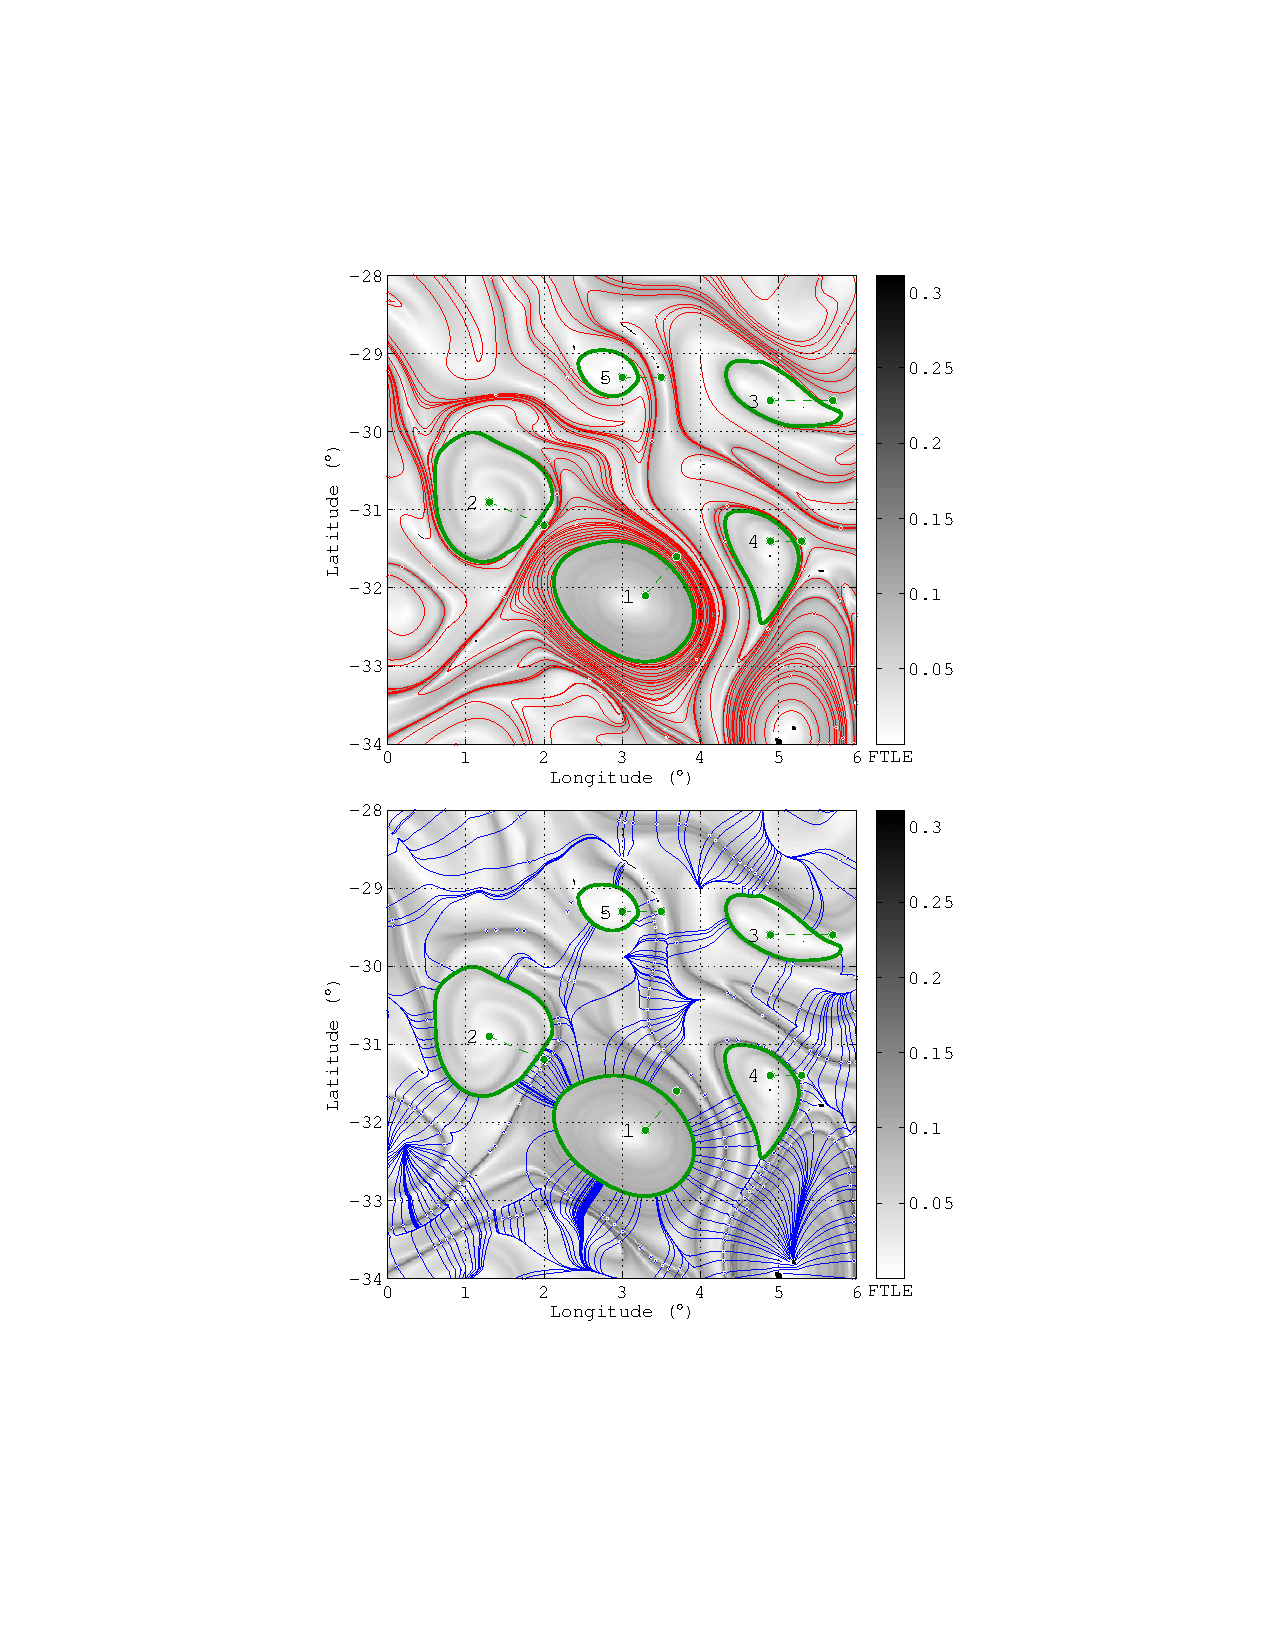
\includegraphics[width=.475\textwidth]{graphics/ocean_dataset/lambda_hyperbolic_lcs}
\end{center}
\caption{
LCSs in the ocean velocity data from satellite altimetry.
Resolution is $[500\times250]$.
Elliptic LCSs are green, shrink line LCSs are red and stretch line LCSs are blue. 
White dots indicate $\lambda_2$ maxima for shrink lines and $\lambda_1$ minima stretch lines.
FTLE shown in the background.
$\lambda=$ 1.00, 1.08, 0.94, 0.90, 1.06
}
\label{f:ocean dataset LCS}
\end{figure}

\section{Conclusions}

We have described a computational toolbox, LCS Tool, that implements recent variational results for Lagrangian Coherent Structures (LCSs) in two-dimensional unsteady flows. We have also demonstrated the performance of LCS Tool on two analytic flow models and a geophysical velocity dataset. The publicly available software library producing these results enables the exploration of variational LCS methods without assuming a detailed knowledge of geodesic LCS theory.

LCS Tool leverages the capabilities of MATLAB. For FTLE based extraction of LCSs, computational performance has received considerable attention \citep{conti12:_gpu_apu_finit_time_lyapun_expon,miron12:_anisot_lagran_coher_struc}.
We think LCS Tool can facilitate similar computational advances for variational LCS methods.
Optimizing computational performance will aid applications to large-scale forecasting applications, such as the tracking of environmental contaminants\citep{olascoaga12:_forec}.

We hope LCS Tool will serve as a foundation for the numerical implementation of recent theoretical advances.
These include the geodesic theory of parabolic LCSs (jet cores)\citep{farazmand14:_shearless} and the variational theory of hyperbolic and elliptic LCSs for three-dimensional flows\citep{blazevski14:_hyper_ellip_trans_barrier_three}.

\section*{Acknowledgements}

\begin{sloppypar}
The altimeter products used in this work are produced by SSALTO/DUACS and distributed by AVISO, with support from CNES, \url{http://www.aviso.oceanobs.com/duacs}.
\end{sloppypar}

\section*{References}

% FIXME Citations without pages (haller15:_langr_coher_struc and karrasch14:_autom_lagran) do not list publication year
\bibliographystyle{elsarticle-num-names} 
\bibliography{main}

\end{document}

% Local Variables:
% ispell-dictionary: "en_GB"
% End:
% LocalWords:  incompressible gyre eigenvector eigenvectors incompressibility dataset datasets LCS LCSs Lyapunov Bickley Rossby timespan variational adaptively vortices parametrise advected minima extremal FTLE MATLAB maxima geostrophic Poincare altimetry zonal
